\documentclass[12pt,a4paper]{book}
\raggedbottom

\usepackage{ugmath}
\usepackage{float}
\usepackage{placeins}
\usepackage[labelfont=bf,labelsep=space]{caption}
\usepackage{pdfpages}
\usepackage{tikz-cd}
\usepackage{amsthm}
\DeclareMathOperator{\rg}{rg}
\renewcommand{\Tr}{\operatorname{Tr}}
\newcommand{\llaves}[1]{\{#1\}}
\newcommand{\parentesis}[1]{\left(#1\right)}
\newcommand{\corchetes}[1]{\left[#1\right]}
\newcommand{\llavesgrande}[1]{\big\{#1\big\}}
\newcommand{\llavesgrandes}[1]{\left\{#1\right\}}
\usepackage{titlesec}


\begin{document}

    \thispagestyle{empty}
    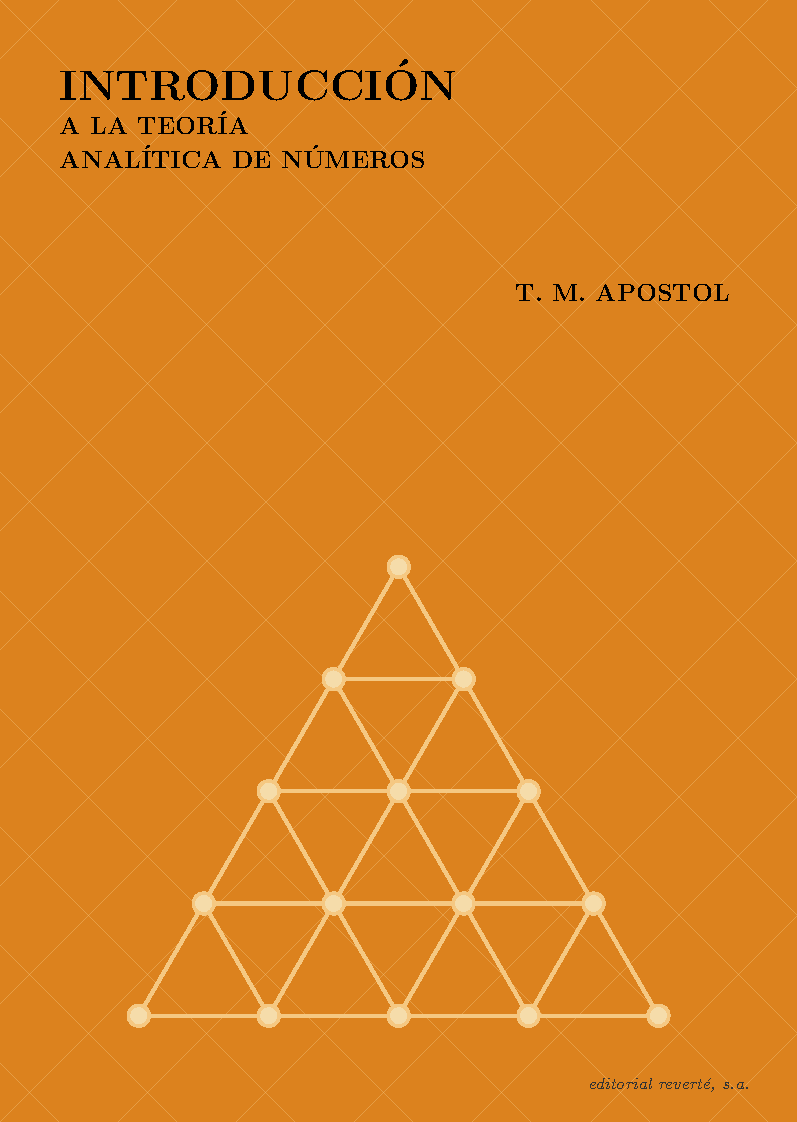
\includepdf[pages=1]{portada_apostol.pdf}

    \begin{titlepage}
    \centering
    \vspace*{3cm}

    {\fontsize{28}{36}\selectfont Introducción\\[6pt]
    a la Teoría\\[6pt]
    analítica de números\par}

    \vspace{2cm}

    {\fontsize{14}{18}\selectfont Tom M. Apostol\par}

    \vfill

    % Logo de Reverté (círculo aproximado si no tienes la imagen)
    % Si tienes el logo como imagen:
    % \includegraphics[width=2.5cm]{reverte_logo.png}
    \tikz\draw[thick] circle (1cm) node {\small\textbf{REVERTÉ}};

    \vspace{0.5cm}

    {\fontsize{11}{14}\selectfont\textbf{EDITORIAL REVERTÉ, S. A.}\par}

    \vspace{0.3cm}

    {\fontsize{8}{10}\selectfont
    Barcelona·Bogotá·Buenos Aires·Caracas·México·Rio de Janeiro\par}

    \vspace{1cm}
    \end{titlepage}

    \setcounter{page}{1}
    \tableofcontents

    \chapter{El teorema fundamental de la Aritmética}

    \section{INTRODUCCIÓN}

    En este capitulo se introducen conceptos básicos de la Teoría elemental de números tales
    como la divisibilidad, el máximo común divisor, y los números primos y compuestos. Los
    resultados principales son el teorema 1.2, que establece la existencia del máximo común
    divisor para todo par de enteros, y el teorema 1.10 (Teorema fundamental de la Aritmética),
    que demuestra que todo entero mayor que 1 se puede representar como prodcuto de factores
    primos de forma única (salvo el orden de los factores). Muchas de las demostraciones utilizan
    la sigueinte propiedad de enteros.

    \textbf{El principio de inducción}. Si $Q$ es un conjunto de enteros tales que
    \begin{enumerate}
        \item[(a)] $1\in Q$.
        \item[(b)] $n\in Q$ implica $n+1\in Q$, 
    \end{enumerate}
    entonces
    \begin{enumerate}
        \item[(c)] todo entero $\geq1$ pertenece a $Q$.
    \end{enumerate}

    Existen, además, otras formulaciones de este principio. Por ejemplo, en (a) podemos
    substituir 1 por un entero cualquiera $k$, siempre que en (c) la desigualdad $\geq1$
    se substituya por $\geq k$. Además (b) se puede substituir por $1,2,3,\dots,n\in Q$
    implica $(n+1)\in Q$.

    Suponemos que el lector se halla familiarizado con este principio así como con su uso en las
    demostraciones de teoremas por inducción. Le suponemos también familiarizado con el siguiente
    principio que es logicamente equivalente al principio de inducción.

    \textbf{El principio de buena ordenación.} Si $A$ es un conjunto no vacio de enteros positivos,
    entonces $A$ posee un elemento minimo.\\
    De nuevo, este principio posee formulaciones equivalentes. Por ejemplo, enteros positivos
    se puede substituir por enteros $\geq k$ para un cierto $k$.

    \section{DIVISIBILIDAD}

    \textbf{Notación.} En este capítulo, las letras latinas minúsculas $a,b,c,d,n,$ etc,
    denotan enteros; pueden ser positivos, negativos, o cero.

    \begin{definicion}[Divisibilidad]
        Diremos que $d$ divide $n$ y escribiremos $d\mid n$ si $n=cd$ para algun $c$.
        Diremos también que $n$ es múltiplo de $d$, que $d$ es un divisor de $n$, o que
        $d$ es un factor de $n$. Si $d$ no divide a $n$ escribiremos $d\nmid n$.
    \end{definicion}

    La divisibilidad establece una relación binaria entre enteros con las siguientes propiedades
    elementales cuyas demostraciones se dejan como ejercicio para el lector, (Salvo indicación
    expresa, las letras $a,b,d,m,n$ del teorema 1.1 representan enteros arbitrarios).

    \begin{teorema}
        La divisibilidad verifica las siguientes propiedades:
        \begin{enumerate}
            \item[(a)] $n\mid n$\hfill \textit{(propiedad reflexiva)}
            \item[(b)] $d\mid n$ y $n\mid m$ implica $d\mid m$\hfill\textit{(propiedad transitiva)}
            \item[(c)] $d\mid n$ y $d\mid m$ implica $d\mid(an+bm)$\hfill\textit{propiedad lineal}
            \item[(d)] $d\mid n$ implica $ad\mid an$\hfill\textit{(propiedad de multiplicación)}
            \item[(e)] $ad\mid an$ y $a\neq0$ implica $d\mid n$\hfill\textit{propiedad de simplificación}
            \item[(f)] $1\mid n$\hfill\textit{(1 divide a todos los enteros)}
            \item[(g)] $n\mid0$\hfill\textit{(cada entero divide a cero)}
            \item[(h)] $0\mid n$ implica $n=0$\hfill\textit{(el cero solo divide al cero)}
            \item[(i)] $d\mid n$ y $n\neq0$ implica $\abs{d}\leq\abs{n}$\hfill\textit{(propiedad de comparación)}
            \item[(j)] $d\mid n$ y $n\mid d$ implica $\abs{b}=\abs{n}$
            \item[(k)] $d\mid n$ y $d\neq0$ implica $(n\mid d)\mid n$          
        \end{enumerate}
    \end{teorema}

    Nota. Si $d\mid n$ entonces $n\mid d$ se llama el divisor conjugado de $d$.

    \section{MÁXIMO COMÚN DIVISOR}

    Si un $d$ divide a dos enteros $a$ y $b$, entonces $d$ se llama

\end{document}